\scanpage{6}

\[
\begin{aligned}
&\deleted{\widetilde L_0=\pi^{-1}(L_0)\subset\widetilde K_0}\\
&\deleted{\widetilde L=T}
\end{aligned}
\]
\diagram{\begin{tikzcd}[ampersand replacement=\&,row sep=0.1em,column sep=1em]
\widetilde K \arrow[rr,"\pi"] \& \& K\\
\cup \& \& \deleted{\unsure{\cup}}\quad\unsure{\supset}\\
\widetilde L \& {}=\pi^{-1}(L)\arrow[r] \& L
\end{tikzcd}}

\[
\left\{\begin{aligned}
|\widetilde K|-|\widetilde L|&\xrightarrow{\sim}|K|-|L|\\
(\widetilde K,\widetilde L)&\text{ est ``pur''}
\end{aligned}\right.
\qquad
\widetilde K=\varinjlim_{x\in K\backslash L}
\underset{\substack{\shortparallel\\ \{y\in K\mid y\leq x\}}}{K_x}
\]

\figure{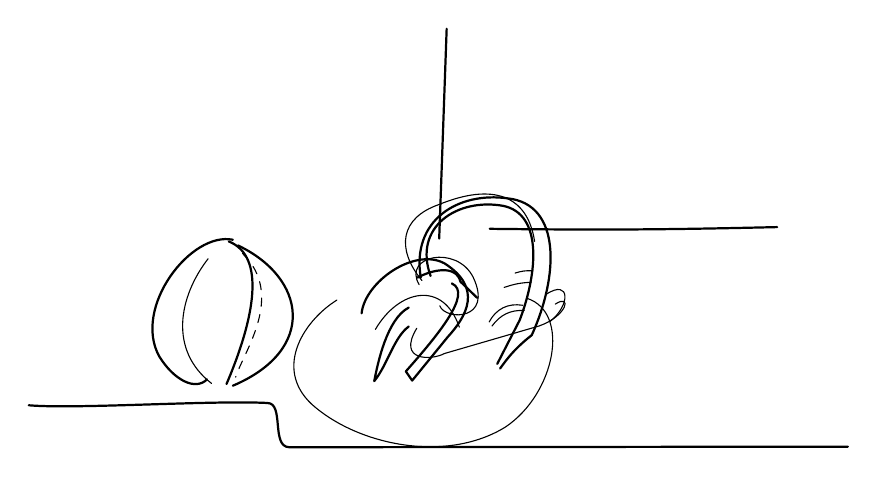
\begin{tikzpicture}[x=0.73cm,y=-0.73cm,line cap=round,line join=round]
\draw[thick] (0.0,2.98) .. controls (0.81,3.05) and (3.19,2.89) .. (4.15,2.94)
 .. controls (4.45,2.94) and (4.21,3.70) .. (4.53,3.71) -- (14.25,3.70);
\draw[thick] (8.02,-0.09) to[bend right=1] (13.02,-0.12);
\draw[thick] (7.27,-3.57)--(7.14,0.08);
\draw[thick] (3.55,0.10) .. controls (2.82,-0.05) and (1.80,1.28) .. (2.27,2.13)
 .. controls (2.53,2.55) and (2.90,2.73) .. (3.10,2.53);
\draw (3.12,0.43) .. controls (2.61,1.09) and (2.43,2.02) .. (3.18,2.60);
\draw[thick] (3.48,0.13) .. controls (4.13,0.39) and (3.93,1.46) .. (3.44,2.61);
\draw[thin,dashed] (3.72,0.34) .. controls (4.47,1.07) and (3.73,2.06) .. (3.60,2.49);
\draw[thick] (3.64,0.20) .. controls (4.82,0.76) and (5.03,2.01) .. (3.55,2.64);
\draw (5.36,1.15) .. controls (4.75,1.53) and (4.23,2.40) .. (4.99,3.02)
 .. controls (5.80,3.69) and (7.28,3.98) .. (8.29,3.36)
 .. controls (9.16,2.78) and (9.43,1.37) .. (8.67,1.12);
\draw[thick] (5.79,1.38) .. controls (5.85,0.83) and (6.71,0.23) .. (7.23,0.51)
 .. controls (7.91,0.94) and (7.61,1.44) .. (7.29,1.79) -- (6.67,2.55)--(6.56,2.39)
 .. controls (7.10,1.78) and (7.73,1.03) .. (7.36,0.86);
\draw (6.03,1.66) .. controls (6.44,0.96) and (7.21,0.80) .. (7.49,1.62);
\draw[thick] (6.61,1.28) .. controls (6.23,1.48) and (6.07,2.25) .. (6.01,2.56)
 .. controls (6.25,2.26) and (6.35,1.80) .. (6.61,1.61);
\draw (6.75,1.64) .. controls (6.40,2.22) and (7.01,2.20) .. (7.23,2.08) -- (8.88,1.60)
 .. controls (9.38,1.42) and (9.45,1.03) .. (9.16,1.22);
\draw (6.79,0.88) .. controls (6.50,0.38) and (7.44,0.18) .. (7.73,0.75)
 .. controls (8.09,1.51) and (7.25,1.51) .. (7.15,1.25);
\draw[thick] (6.76,0.76) .. controls (7.00,0.63) and (7.43,0.52) .. (7.51,0.83)--(7.80,1.11);
\draw[thin] (6.84,0.81) .. controls (6.38,0.25) and (6.47,-0.28) .. (7.13,-0.51)
 .. controls (8.08,-0.90) and (8.68,-0.67) .. (8.80,0.13);
\draw[thick] (6.82,0.76) .. controls (6.65,-0.24) and (7.47,-0.74) .. (8.33,-0.62)
 .. controls (9.27,-0.52) and (9.22,0.73) .. (8.75,1.76) to[bend right=8] (8.20,2.34);
\draw[thick] (6.99,0.73) .. controls (6.68,-0.13) and (7.46,-0.63) .. (8.25,-0.49)
 .. controls (8.95,-0.35) and (8.85,0.69) .. (8.54,1.50) -- (8.15,2.26);
\draw (8.01,1.53) to[bend left=36] (8.59,1.24) (8.06,1.60) to[bend left=28] (8.62,1.33)
 (8.27,0.93) to[bend left=8] (8.74,0.84) (8.46,0.68) to[bend left=10] (8.77,0.64)
 (9.00,1.05) .. controls (9.43,0.77) and (9.42,1.25) .. (9.07,1.52);
\end{tikzpicture}}
% crop-candidate: scan 6

% slanted
\margin{$\begin{aligned}
|x'|,|y'|&\leq\sqrt{x^{\prime\unsure{2}}\unsure{+|-}y^{\prime 2}}\leq |x'|+|y'|\\
\int|x'|,\int|y'|&\leq\int -\leq\int|x'|+\int|y'|
\end{aligned}$}

\[
\sum_{\widetilde K_i}(X_i,\partial X_i)=|\widetilde K_i|
\]

\figure{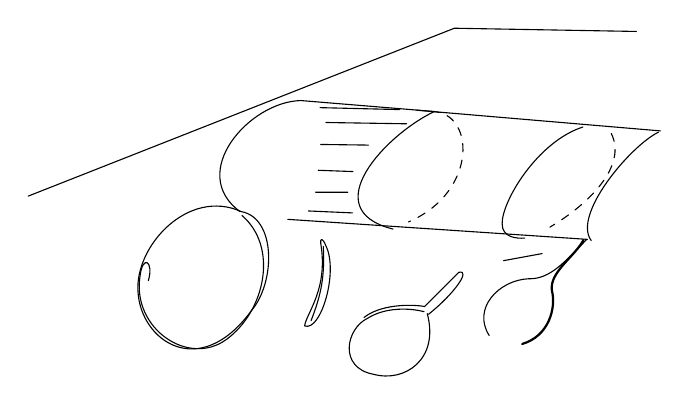
\begin{tikzpicture}[x=0.82cm,y=-0.82cm,line cap=round,line join=round]
\draw[thin] (0,2.35)--(6.6,-0.25)--(9.42,-0.20);
\draw[thin] (3.28,2.59) .. controls (2.46,1.99) and (3.42,0.89) .. (4.22,0.87)
 --(6.29,1.04) .. controls (5.55,1.39) and (4.43,2.56) .. (5.65,2.86);
\draw (4.02,2.71) --(8.66,3.02) (6.02,1.02)--(9.79,1.34);
\draw (8.59,1.28) .. controls (7.88,1.51) and (7.33,2.44) .. (7.34,2.78)
 .. controls (7.34,2.99) and (7.56,3.01) .. (7.69,3.00);
\draw (9.76,1.36) .. controls (9.33,1.57) and (8.42,2.64) .. (8.72,3.04);
\draw[dashed,thin] (6.24,1.04) .. controls (6.92,1.03) and (6.98,2.28) .. (5.89,2.75)
 (9.03,1.38) .. controls (9.28,1.88) and (8.69,2.47) .. (8.08,2.83);
\draw[thin] (4.52,0.98)--(5.75,1.01) (4.61,1.21)--(5.86,1.23) (4.53,1.55)--(5.27,1.56)
 (4.49,1.95)--(5.03,1.97) (4.45,2.29)--(4.95,2.29) (4.34,2.58)--(5.02,2.61);
\draw (3.30,2.59) .. controls (3.84,2.69) and (3.83,3.68) .. (3.46,4.12)
 .. controls (2.65,5.23) and (1.74,4.59) .. (1.70,3.83) .. controls (1.65,3.12) and (2.48,2.22) .. cycle;
\draw[thin] (3.31,2.65) .. controls (3.88,3.14) and (3.67,4.13) .. (3.07,4.57)
 .. controls (2.48,5.00) and (1.61,4.40) .. (1.73,3.60) .. controls (1.77,3.24) and (1.95,3.36) .. (1.86,3.66);
\draw (4.53,3.08) .. controls (4.65,3.79) and (4.31,4.16) .. (4.28,4.36)
 .. controls (4.53,4.46) and (4.81,3.52) .. (4.61,3.12) .. controls (4.56,2.99) and (4.52,3.00) .. cycle;
\draw[thin] (4.57,3.13) to[bend left=12] (4.38,4.28);
\draw (5.20,4.23) .. controls (5.45,4.03) and (5.91,4.02) .. (6.14,4.06)
 --(6.67,3.53) .. controls (6.86,3.49) and (6.60,3.86) .. (6.20,4.18);
\draw (6.18,4.17) .. controls (6.37,4.88) and (5.83,5.24) .. (5.35,5.11)
 .. controls (4.80,5.01) and (4.92,4.40) .. (5.26,4.24) .. controls (5.53,4.07) and (5.90,4.08) .. (6.13,4.14);
\draw (7.14,4.51) .. controls (6.87,4.09) and (7.29,3.65) .. (7.75,3.63)
 .. controls (8.08,3.64) and (8.31,3.37) .. (8.65,3.02);
\draw[thick] (7.65,4.64) .. controls (8.06,4.52) and (8.18,4.09) .. (8.11,3.81)
 .. controls (8.07,3.53) and (8.46,3.29) .. (8.60,3.03);
\draw (7.36,3.35)--(7.96,3.24);
\end{tikzpicture}}
% crop-candidate: scan 6
% archive sheet number: 5
